%%%%%   INTRODUCCIÓN   %%%%%
%---------------------------------------------------------
%\section{Objetivo del documento}
%    El presente documento \varCveDocumento\ tiene como objetivo mostrar en detalle los requerimientos funcionales y no funcionales, modelos de información, reglas de negocio, modelos de comportamiento, casos de uso e interfaces correspondientes a cada uno de los módulos propuestos para esta etapa.

\section{Antecedentes}

En la antigüedad se realizaban procedimientos que carecían de valor terapéutico y muchos de estos tratamientos mas que ayudar al paciente complicaban la situación.\\
Fue hasta el siglo XX en que la medicina empezó a contar con un arsenal terapéutico que ya tenia una efectividad comprobada.\\
Al día de hoy se cuenta con un mayor conocimiento de las enfermedades, de como combatirlas, de saber interpretar los síntomas y que escenarios fomentan a su desarrollo. Como es mencionado en el estudio " El tratamiento medico: Experiencia, base teórica y método " en la segunda mitad del siglo pasado se desarrollo la metodología de los ensayos clínicos aleatorios, que es hasta el momento el recurso mas confiable para conocer la efectividad real de cualquier tipo de tratamientos, aunque a pesar de la gran cantidad de ensayos clínicos realizados, mucho mas de la mitad de los tratamientos que se practican no han sido sometidos a esa prueba, lo cual no impide que sean utilizados siempre y cuando, haya un base teórica aceptable y lógica que apoye sus beneficios.\\
La medicina es una ciencia inexacta ya que esta cuenta con el factor biológico de cada individuo es por eso que los tratamientos médicos necesitan contar un metodología que se encargara de sistematizar y ordenar los pasos que tendrán de base para tener un terapéutica racional.
El origen de cualquier metodología medica tiene sustento en la guía propuesta en la Universidad de Groningen en Holanda y que con el apoyo de la Organización Mundial de la salud presentan 6 pasos que se espera que se acondicionen a las condiciones de trabajo.

Cuando un profesional de la salud esta por ejecutar una prescripción medica debe de ser consciente que un tratamiento medico no debe de ser un reflejo de las quejas del paciente, ni que por cada síntoma se tendrá que prescribir un medicamento, o que dos pacientes pueden ser ajustados para llevar el mismo procedimiento clínico.\\
Muchas veces se puede llegar a tener un prescripción inadecuada de medicamentos, del uso excesivo de medicamentos por complacencia del cliente.  
Los pasos que se recomiendan para el profesional de la salud son los siguientes:
\begin{itemize}
	\item Definir el o los problemas de la salud del paciente
	\item Especificar los objetivos del tratamiento(alcance del tratamiento)
	\item Diseñar el esquema terapéutico mas apropiado para las necesidades del paciente
	\item Brindar información, instrucciones y advertencias
	\item Supervisar la evolución del tratamiento	
\end{itemize}




%\section{Contexto de trabajo}
%
%
%Se trabajara una vez que se haya terminado el marco teórico.
%
%Los seres humanos somos vulnerables a contraer distintos tipos de enfermedades por malos hábitos, por la poca actividad física, debilidades en el sistema inmunológico, entre muchas cosas más, provocando así la necesidad de acudir con un doctor que nos dará un tratamiento médico en donde con un conjunto de procedimientos higiénicos, farmacológicos, de rehabilitación y de acuerdo a las aflicciones y síntomas que presentemos se esperara curar o disminuir el impacto en nuestra salud.


\section{Problemática}


Los tratamientos médicos son un conjunto de procedimientos higiénicos, farmacológicos y de rehabilitación que son recetados por un profesional de la salud para el bienestar del paciente. Por la naturaleza de los tratamientos médicos y su complejidad al administrarlo, la similitud en los múltiples medicamentos en el mercado, su poca claridad en las etiquetas, entre muchas otras cosas más conlleva a que se produzcan erores de medicación y que éstos a su vez provoquen efectos adversos a los pacientes. De acuerdo a la \textbf{NCCMERP} (National Coordinating Council for Medication Error Reporting and Prevention) define los errores de medicación como "cualquier incidente prevenible que puede causar daño al paciente o dar lugar a una utilización inapropiada de los medicamentos". Dichos errores de medicación podrían ser solventados con el uso de las nuevas tecnologías de información.


\section{Solución propuesta por otras aplicaciones}

En la tabla \ref{SolucionesProp} se muestran las aplicaciones que están enfocadas al ámbito de la salud y que intentan cumplir con la problemática planteada pero que ninguna de ellas es capaz de satisfacer al cien por ciento.

\begin{table}[H]
	\resizebox{18cm}{!} {
	
	\begin{tabular}{|l|c|c|c|c|c|c|c|}
		\hline
		\multicolumn{1}{|c|}{Aplicación} & Multiplataforma & \begin{tabular}[c]{@{}c@{}}Notificaciones\\ de\\ Medicamentos\end{tabular} & \begin{tabular}[c]{@{}c@{}}Alertas\\ a contactos\\ de Emergencia\end{tabular} & \begin{tabular}[c]{@{}c@{}}Información\\ de\\ Medicamentos\end{tabular} & \begin{tabular}[c]{@{}c@{}}Múltiples\\ perfiles\end{tabular} & \begin{tabular}[c]{@{}c@{}}Historial\\ de\\ Medicamentos\end{tabular} & \begin{tabular}[c]{@{}c@{}}Captura\\ de\\ tratamiento\end{tabular} \\ \hline
		RecuerdaMed                      & Sí              & Sí                                                                         & No                                                                            & No                                                                      & Sí                                                           & No                                                                    & Sí                                                                 \\ \hline
		Dosecast                         & Sí              & Sí                                                                         & No                                                                            & No                                                                      & No                                                           & \begin{tabular}[c]{@{}c@{}}Sí\\ (Solo Premium)\end{tabular}           & Sí                                                                 \\ \hline
		Medisafe                         & Sí              & Sí                                                                         & No                                                                            & No                                                                      & \begin{tabular}[c]{@{}c@{}}Sí\\ (Solo Premium)\end{tabular}  & No                                                                    & Sí                                                                 \\ \hline
		PillManager                      & Sí              & No                                                                         & No                                                                            & No                                                                      & No                                                           & Sí                                                                    & Sí                                                                 \\ \hline
		PharApp                          & Sí              & No                                                                         & No                                                                            & Sí                                                                      & No                                                           & No                                                                    & No                                                                 \\ \hline
		Capzule                          & Sí              & Sí                                                                         & No                                                                            & No                                                                      & No                                                           & Sí                                                                    & Sí                                                                 \\ \hline
		Andaman7                         & Sí              & No                                                                         & No                                                                            & No                                                                      & Sí                                                           & Sí                                                                    & Sí                                                                 \\ \hline
		GenieMD                          & Sí              & Sí                                                                         & No                                                                            & Sí                                                                      & Sí                                                           & No                                                                    & Sí                                                                 \\ \hline
	\end{tabular}
	}
\caption{Soluciones propuestas por otras aplicaciones}
\label{SolucionesProp}
\end{table}

	
\section{Solución propuesta}

Por lo visto en la seccion anterior, en este trabajo terminal se propone una aplicacion movil llamada Rem-Pills que tiene como principal objetivo cumplir con la problematica y para poder cumplir con esta se porponen las siguientes caracteristicas.
\begin{itemize}
	\item Multiplataforma que funcionara en el sistema operativo Android con la version 5.0(Lollipop) y tambien funcionara en el sistema operativo iOS con la vesion 10.
	
	\item Una interfaz intuitiva que ayude a mejorar los niveles de usabilidad en los usuarios en el momento en que agreguen sus tratamientos medicos.

	\item Programación de recordatorios los cuales contaran con notificaciones audiovisuales.
	
	\item Múltiples perfiles.
	
	\item Alertas a los contactos de emergencia que serán activadas cuando una notificación no sea silenciada después de 3 avisos.
	
	\item Información acerca de la utilización, efectos secundarios y principales usos de los medicamentos.
	
	\item Historial semanal, mensual o anual de los medicamentos, tratamientos clinicos y datos relevantes de la salud del usuario.
	
\end{itemize}

%En la figura \ref{label} se muestra el diagrama de la propuesta de solución

%Por lo visto anteriormente se propone una aplicacion movil llamada Rem-Pills, que tiene como principal objetivo satisfacer la problematica planteada
%
%Por todo lo anterior se propone una aplicacion movil que llamaremos Rem-Pills, para la ayuda en el segu medicos que se 

%\section{Solución propuesta}
%Eso se encuentra en la introducción. ¿Lo dividimos o quitamos esta sección?
%
%\section{Justificación}
%
%
%\section{Objetivos}
%\subsection{Objetivo general}
%
%\subsection{Objetivos específicos}
%	\begin{itemize}
%		\item 
%	\end{itemize}	
%
%%\section{Productos o resultados esperados}
%%\textbf{Esta sección está en el protocolo pero no nos la dijo el profesor. ¿La dejamos?}
%%
%%En la Figura \ref{fig:IntroduccionArqui} se muestra la arquitectura del sistema, la cual se conforma de cuatro etapas las cuales se describen a continuación:
%
%%\begin{enumerate}
%%	\item \textbf{Sensores.} En esta etapa se tomarán las mediciones de los signos vitales  con los sensores determinados durante el análisis.
%%	\item \textbf{Digitalización.} Una vez obtenidas las mediciones de los sensores, éstas pasarán a ser digitalizadas mediante un dispositivo digital programable para obtener la señal procesada.
%%	\item \textbf{Envío de datos.} Con los datos obtenidos en la etapa anterior, se realizará el envío a un teléfono celular.
%%	\item \textbf{Recepción de datos.}  Las señales procesadas de los signos vitales serán recibidas en el teléfono celular en donde se guardará el historial de los datos para futuras consultas.
%%\end{enumerate}
%%
%%De la realización de este Trabajo Terminal se obtendrán los siguientes productos:
%%
%%\begin{enumerate}
%%	\item Código.
%%	\item Sistema embebido.
%%	\item Aplicación móvil.
%%	\item Documentación técnica del sistema.
%%	\item Manual de usuario.
%%\end{enumerate}
%%
%%\begin{figure}[htbp!]
%%	\centering
%%	\fbox{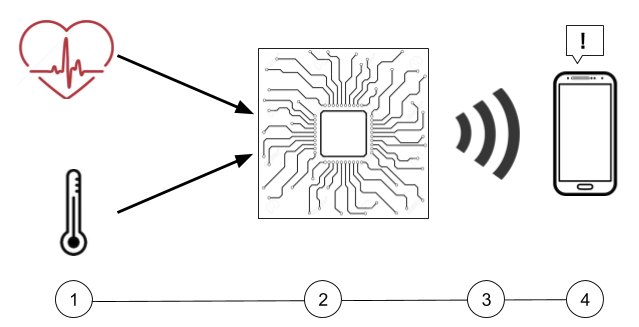
\includegraphics[width=0.8\textwidth]{images/introduccion/arquitectura.png}}
%%	\caption{Arquitectura del sistema.}
%%	\label{fig:IntroduccionArqui}
%%\end{figure}
%
%\section{Metodología}
%%Para la realización del trabajo terminal se propone emplear el Modelo en V ya que ofrece una visión detallada de los diversos pasos e interacciones relacionados con el proceso de desarrollo y puede considerarse como un flujo de trabajo comúnmente utilizado. En la Figura \ref{fig:IntroduccionMetodologia} se muestran las principales actividades abordadas por el método. Convencionalmente, el lado izquierdo del modelo representa las fases del diseño del sistema, mientras que el lado derecho representa las fases de validación y verificación del sistema integrado.
%%
%%\TODO \textbf{Cambiar resolución de imagen.}
%%\begin{figure}[htbp!]
%%	\centering
%%	\fbox{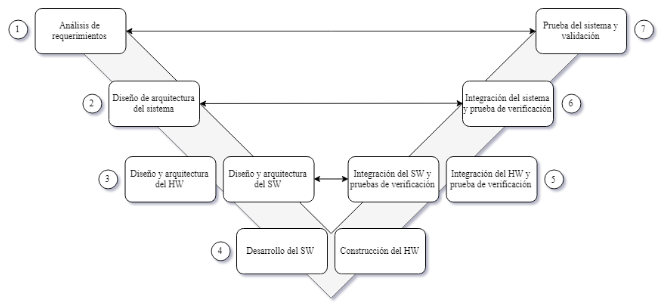
\includegraphics[width=\textwidth]{images/introduccion/metodologia.png}}
%%	\caption{Fases del modelo en V.}
%%	\label{fig:IntroduccionMetodologia}
%%\end{figure}
%%
%%El desarrollo se llevará a cabo en las siguientes etapas:
%%
%%\begin{enumerate}
%%	\item Análisis de requerimientos. Esta fase consiste en establecer qué debe hacer el sistema ideal, sin determinar cómo se construirá o diseñará el software. 
%%	\item Diseño de arquitectura del sistema. El diseño de la arquitectura del sistema consiste en varios pasos, como refinar las funciones del sistema y asignarlas a los diferentes componentes del sistema que pueden ser físicos o de hardware.
%%	\item Diseño de arquitectura de SW y HW. En esta fase del desarrollo del sistema, se diseña el hardware y el software de los diversos elementos que constituyen los componentes del sistema global. Las actividades que se aplican son similares a las realizadas en la fase anterior, pero centrándose en un componente específico del sistema: 
%%		\begin{itemize}
%%			\item Refinamiento de los requerimientos funcionales y no funcionales del hardware y software.
%%			\item Asignación de las funciones del software a los componentes de hardware.
%%		\end{itemize}
%%	\item Desarrollo del SW y Construcción del HW. Una vez que todos los componentes del sistema están diseñados, los elementos de hardware se construyen físicamente y los módulos de software son desarrollados en paralelo, y finalmente integrados con el hardware. Al final de este paso, los elementos de software y hardware deben estar disponibles para las actividades de verificación. Pueden realizarse algunas pruebas unitarias en paralelo con la implementación.
%%	\item Integración y verificación del SW y HW. En este paso se ensamblan los componentes de hardware y software. Las pruebas de verificación se ejecutan para comprobar el cumplimieno de los objetivos de diseño.
%%	\item Integración del sistema y prueba de verificación. En este paso, los elementos del sistema (HW, SW) se combinan y tiene lugar la verificación de los requisitos del sistema. 
%%	\item Prueba del sistema y validación. Esta última de verificación tiene como objetivo validar si los resultados obtenidos cumplen con los requerimientos.
%%\end{enumerate}
%
%%\section{Estructura del documento}
%%	\textbf{Creo que estaría bien agregar la descripción de los capítulos que abarca el documento pero no sé si aquí esté bien.}